\section{Prospetto economico}
In questa sezione vengono presentati, per ciascuna fase del progetto, i prospetti economici relativi alle ore preventivate per i ruoli. Il costo relativo alle fasi di \textbf{Analisi dei Requisiti} e \textbf{Incremento fase di Analisi} non sono a carico del committente quindi non sono considerate nel calcolo delle ore totali da retribuire.

\subsection{Analisi}
Nella fase di \textbf{Analisi} le ore sono suddivise nel modo seguente:
\begin{table}[H]
  \centering
  \begin{tabular}{|c|c|c|}
  \hline
  \textbf{Ruolo} &
  \textbf{Ore} &
  \textbf{Costo} \\
  \hline
  Responsabile & 26 & 780\\
  \hline
  Amministratore & 21.5 & 430\\
  \hline
  Analista & 63 & 1575\\
  \hline
  Progettista & 0 & 0 \\
  \hline
  Verificatore & 33 & 495\\
  \hline
  Programmatore & 0 & 0 \\
  \hline
   \textbf{Totale} & \textbf{143.5} & \textbf{3280} \\
    \hline
  \end{tabular}
  \caption{Costo per ruolo, fase di Analisi}
\end{table}

I seguenti grafici mostrano rispettivamente come abbiano influito per ore e costi, sul totale, i ruoli nella fase di \textbf{Analisi}.
\begin{figure}[H]
\centering
\scalebox{0.6}{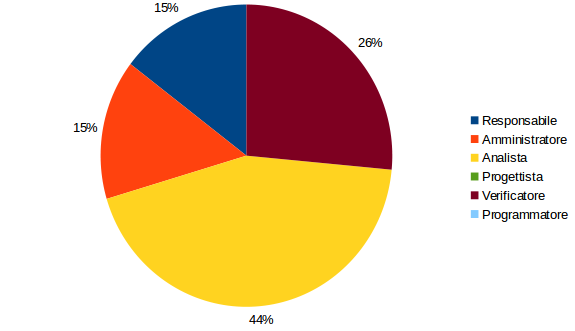
\includegraphics{img_peconomico/oreAnalisi.png}}
\caption{Ore per ruoli, fase di Analisi}
\end{figure}

\begin{figure}[H]
\centering
\scalebox{0.6}{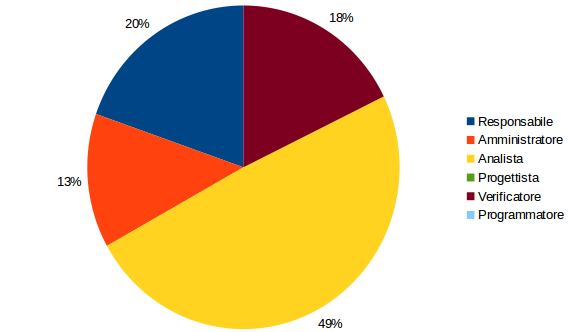
\includegraphics{img_peconomico/costiAnalisi.png}}
\caption{costi per ruoli, fase di Analisi}
\end{figure}
\subsection{Incremento fase di Analisi}
\subsection{Progettazione Architetturale}
\subsection{Progettazione di dettaglio e codifica}
\subsection{Verifica e Validazione}
\subsection{Totale}





